\documentclass[../homework.tex]{subfiles}

\pagestyle{fancy}
\fancyhf{}
\rhead{Hanzhi Zhou}
\lhead{Physics 2415 Homework}
\cfoot{\thepage}

\begin{document}
\subsection{Problem 9.1}
\subsubsection*{a)}
\begin{figure}[H]
    \centering
    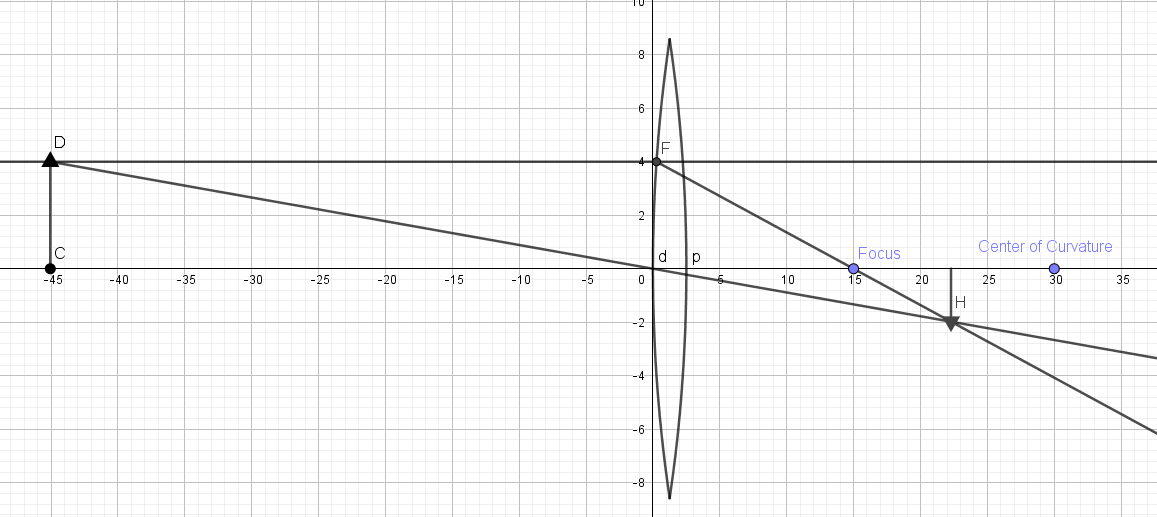
\includegraphics[width=\columnwidth]{p1-a.png}
\end{figure}
\begin{equation*}
    d_i = \left(\frac{1}{15} - \frac{1}{45}\right)^{-1} = \frac{45}{2}
\end{equation*}
\begin{equation*}
    M = -\frac{45/2}{45} = -\frac{1}{2} 
\end{equation*}
The image is real and inverted.

\subsubsection*{b)}
\begin{figure}[H]
    \centering
    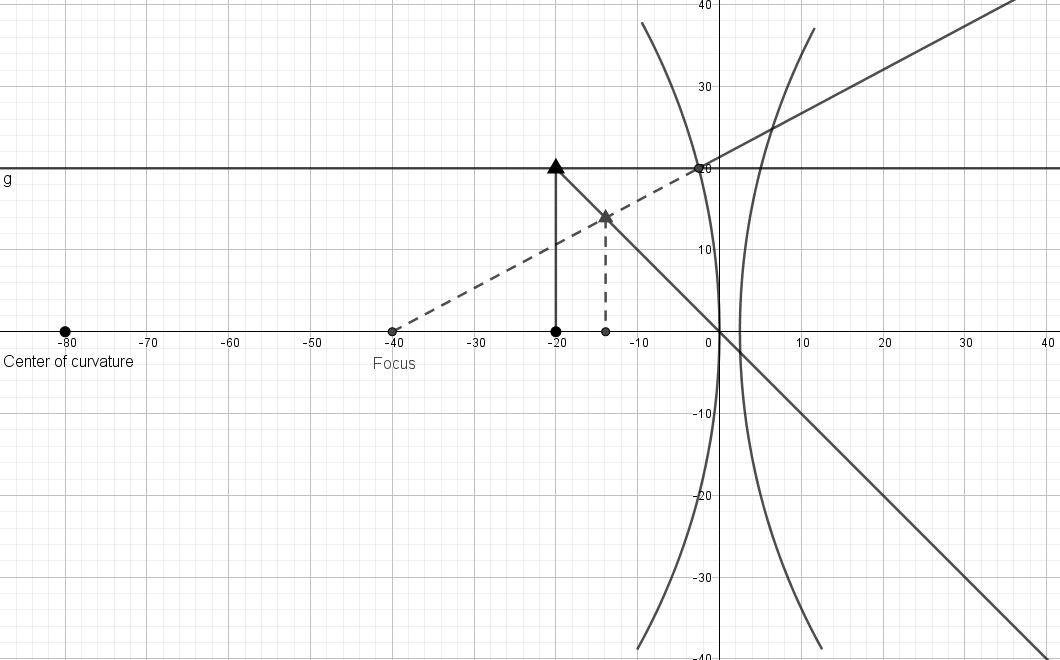
\includegraphics[width=\columnwidth]{p1-b.png}
\end{figure}
\begin{equation*}
    d_i = \left(\frac{1}{-40} - \frac{1}{20}\right)^{-1} = -\frac{40}{3}
\end{equation*}
\begin{equation*}
    M = -\frac{-40/3}{20} = \frac{2}{3} 
\end{equation*}
The image is virtual and upright.

\subsubsection*{c)}
\begin{figure}[H]
    \centering
    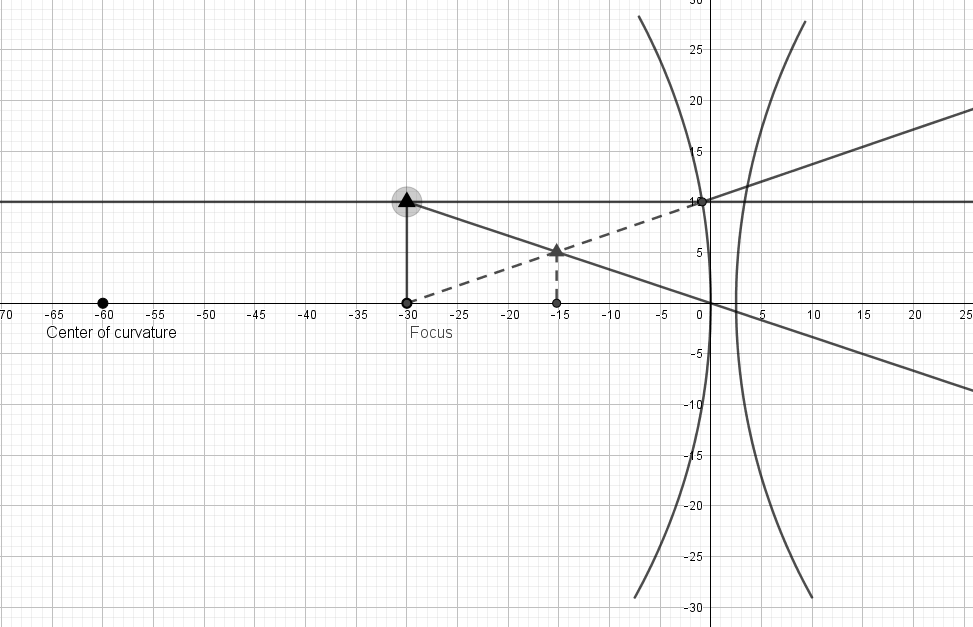
\includegraphics[width=\columnwidth]{p1-c.png}
\end{figure}
\begin{equation*}
    d_i = \left(\frac{1}{-30} - \frac{1}{30}\right)^{-1} = -15
\end{equation*}
\begin{equation*}
    M = -\frac{-15}{30} = \frac{1}{2}
\end{equation*}
The image is virtual and upright.

\subsubsection*{d)}
\begin{figure}[H]
    \centering
    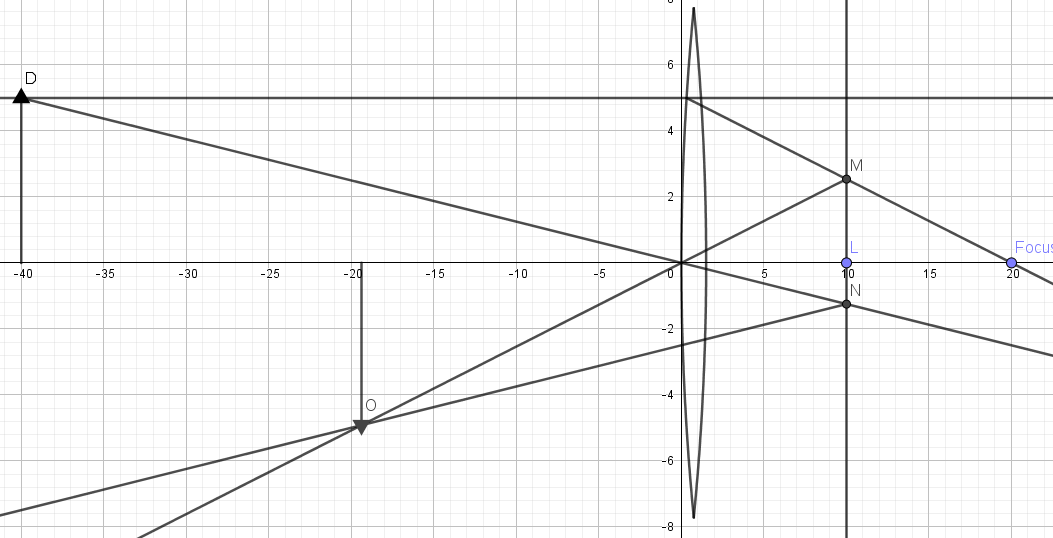
\includegraphics[width=\columnwidth]{p1-d.png}
\end{figure}
After the converging lens,
\begin{equation*}
    d_i = \left(\frac{1}{20} - \frac{1}{40}\right)^{-1} = 40
\end{equation*}
\begin{equation*}
    M = -\frac{40}{40} = -1
\end{equation*}
For the mirror, $d_o = -40 + 10 = -30$, since the object is at the opposite side of the incoming rays. Therefore,
\begin{equation*}
    d_i = d_o = -30
\end{equation*}
Because $d_i$ is negative, the object is at the same side as the incoming rays. The final position of the object is at the left of converging lens. We need to add 10cm to get the final position of the image: 20cm left to the converging lens.

Since the mirror won't change the magnification, the final magnification is $-1$, giving an inverted real image of the same size.
\end{document}